%% OJEPN article template for LaTeX
%% Licence: Creative Commons Attribution Share-Alike 4.0
%% Author:  Andy J. Wills
%% Adapted from a Creative Commons template by Jonathan Baron

\documentclass[twocolumn]{article}
\usepackage[utf8]{inputenc}
\usepackage[T1]{fontenc}
\usepackage[english]{babel}
\usepackage{ifpdf,amsmath,amsthm,amssymb,amsfonts,newtxtext,newtxmath} 
\usepackage{array,graphicx,dcolumn,multirow,hevea,abstract,hanging}
\usepackage[labelfont=sc,textfont=sf]{caption}
\usepackage[colorlinks=true,linkcolor=black,anchorcolor=black,citecolor=black,filecolor=black,menucolor=black,runcolor=black,urlcolor=black,hyperfootnotes=false,breaklinks=true]{hyperref}
\urlstyle{rm}
\usepackage[hyphenbreaks]{breakurl}
%\usepackage{natbib} % must come afer hyperfootnotes
%\setlength{\bibsep}{0pt}
\usepackage{booktabs} % \toprule \midrule \bottomrule \cmidrule(lr){a-b}
% define centered and ragged columns:
\newcolumntype{L}[1]{>{\raggedright\arraybackslash }p{#1}} % can use m{}
\newcolumntype{C}[1]{>{\centering\arraybackslash }p{#1}}
\newcolumntype{R}[1]{>{\raggedleft\arraybackslash }p{#1}}
\newcolumntype{d}[1]{D{.}{.}{#1}} % d{3.2} for 3 places on l, 2 on r
\newcommand{\mc}{\multicolumn}
\topmargin=-.3in \oddsidemargin=-.1in \evensidemargin=-.1in \textheight=9in \textwidth=6.8in
\setlength\tabcolsep{1mm}
\setlength\columnsep{5mm}
\setlength\abovecaptionskip{1ex}
\setlength\belowcaptionskip{.5ex}
\setlength\belowbottomsep{.3ex}
\setlength\lightrulewidth{.04em}
\renewcommand\arraystretch{1.2}
\renewcommand{\topfraction}{1}
\renewcommand{\textfraction}{0}
\renewcommand{\floatpagefraction}{.9}
% \renewcommand{\baselinestretch}{1.00} \large\normalsize % for fixing spaces
\widowpenalty=1000
\clubpenalty=1000
\setlength{\parskip}{0ex}
\let\tempone\itemize
\let\temptwo\enditemize
\let\tempthree\enumerate
\let\tempfour\endenumerate
\renewenvironment{itemize}{\tempone\setlength{\itemsep}{0pt}}{\temptwo}
\renewenvironment{enumerate}{\tempthree\setlength{\itemsep}{0pt}}{\tempfour}

%%%%%%%%%%%%%%%%%%%%%%%%%%%%%%%%%%%%%%%%%%%%%%%%%%%%%%%%%%%%%%%%%%%%%
\setcounter{page}{1} % start with first page

\title{Representing uncertainty in the Rescorla-Wagner model: Blocking, the redundancy effect, and outcome base rate}

\author{
Stuart G. Spicer\thanks{School of Psychology, University of Plymouth, U.K. Email: stuart.spicer@plymouth.ac.uk}
\and 
  Andy J. Wills\footnotemark[1] % indicates same as 1st thanks
\and
  Peter M. Jones\footnotemark[1] % indicates same as 1st thanks
  \and
  Chris J. Mitchell\footnotemark[1] % indicates same as 1st thanks
  \and
  Lenard Dome\footnotemark[1] % indicates same as 1st thanks
}


\date{} % leave empty
\begin{document} % goes here

% fill in short title
\newcommand{\jhead}{Open Journal of Experimental Psychology and Neuroscience, 2021}
\newcommand{\jdate}{Vol.~1}
\pagestyle{myheadings} \markright{\protect\small \jhead, \jdate \hfill REPRESENTING UNCERTAINTY \qquad}
\begin{htmlonly}
\end{htmlonly}
%\begin{latexonly}
\twocolumn[
\vspace{-.3in}
{\small \jhead, \jdate, pp.\ 14--XX \hfill \url{https://doi.org/10.46221/ojepn.2021.6623}}
%\end{latexonly}

\maketitle

%\begin{latexonly}
\vspace{-3mm}
\begin{onecolabstract}
%\end{latexonly}
It is generally assumed that the Rescorla and Wagner (1972) model
adequately accommodates the full results of simple cue competition
experiments in humans (e.g. Dickinson et al., 1984), while the Bush and
Mosteller (1951) model cannot. We present simulations that demonstrate
this assumption is wrong in at least some circumstances. The
Rescorla-Wagner model, as usually applied, fits the full results of a
simple forward cue-competition experiment no better than the
Bush-Mosteller model. Additionally, we present a novel finding, where
letting the associative strength of all cues start at an intermediate
value (rather than zero), allows this modified model to provide a better
account of the experimental data than the (equivalently modified)
Bush-Mosteller model. This modification also allows the Rescorla-Wagner
model to account for a redundancy effect experiment (Uengoer et al.,
2013); something that the unmodified model is not able to do.
Furthermore, the modified Rescorla-Wagner model can accommodate the
effect of varying the proportion of trials on which the outcome occurs
(i.e. the base rate) on the redundancy effect (Jones et al., 2019).
Interestingly, the initial associative strength of cues varies in line
with the outcome base rate. We propose that this modification provides a
simple way of mathematically representing uncertainty about the causal
status of novel cues within the confines of the Rescorla-Wagner model.
The theoretical implications of this modification are discussed. We also
briefly introduce free and open resources to support formal modelling in
associative learning.

\smallskip
\noindent
Keywords: associative learning, prediction error, uncertainty,
modelling, blocking, redundancy effect, open science.

%\begin{latexonly}
\end{onecolabstract}\bigskip
]
%\end{latexonly}

{\renewcommand{\thefootnote}{}
\footnotetext{ % note blank lines above and below acknowledgment
Copyright: \copyright\ 2021.
The authors license this article under the terms of the
\href{http://creativecommons.org/licenses/by/3.0/}{Creative Commons
  Attribution Share-Alike 4.0 License.}
}}

\saythanks

\setlength{\baselineskip}{12pt plus.2pt}

\section{Introduction}

Blocking (Kamin, 1969) is a type of cue competition that occurs when
learning about one cue is apparently restricted by the simultaneous
presence of another cue that has also been trained separately. For
example, if a single cue is followed by an outcome (A+), and a
separately-encountered compound containing that cue is followed by the
same outcome (AX+), then learning about X is restricted (N.B. letters
represent cues and + or - represents the presence or absence of the
outcome). In humans, learning is often tested by asking participants to
rate the likelihood of an outcome such as stomach ache, on the basis of
specific cues such as foods (e.g. Jones et al., 2019). Participants rate
blocked cues as a less likely cause of the outcome than an appropriate
control (e.g. Y following B- BY+ training).

Early models of associative learning were unable to account for
blocking. In particular, the associative learning model developed by
Bush and Mosteller (1951) uses an individual prediction error, which
means that any change in the strength of an association between a cue
and an outcome is governed by the size of the error between the outcome
that occurs and the outcome predicted by that cue alone. For example, if
you predict that a certain type of food is safe to eat, but you
subsequently suffer an allergic reaction after eating that food, then
there will be a large prediction error. Once you have learned that this
type of food is not safe to eat, there will be no error, and learning
will be at asymptote. According to the Bush-Mosteller model, learning
updates as follows:

\begin{equation}
  \Delta V_{x} = \alpha_{x}L(\lambda-V_{x})
\end{equation}

In Equation 1, associative strength is denoted by V, where
$\Delta V_{x}$ is the change in associative strength for cue X, and
$V_{x}$ is the current associative strength of cue X. The cue
salience is represented by $\alpha$ and the outcome learning rate is
represented by $L$. The asymptote of learning is represented by $\lambda$. The
individual prediction error means that the model cannot account for
blocking, as this effect is driven by the interference of simultaneously
encountered cues. To overcome this, Rescorla and Wagner (1972) proposed
a model with an overall prediction error, in which any change in
associative strength is governed by the error between the outcome that
occurs and the outcome predicted by all simultaneously present cues:

\begin{equation}
 \Delta V_{x} = \alpha_{x}L(\lambda - \Sigma V_{x})
\end{equation}

The only change is that $\Sigma V$has been incorporated as the overall
associative strength of all simultaneously-present cues. The model can
account for blocking because A takes up all the available associative
strength on the A+ trials, meaning that there is no available
associative strength for X to acquire on the AX+ trials (assuming
learning is at asymptote).

Dickinson et al. (1984) provided one of the first experimental
demonstrations of blocking in humans. The Rescorla and Wagner (1972)
model is widely assumed to adequately explain the full data of such
experiments, whilst also providing a better account than Bush and
Mosteller's (1951) model. In our first simulation, we conducted a
model-fitting procedure on the full data of a simple forward cue
competition blocking experiment (a standard design incorporating
blocking, a control and filler cues), using both models. It is worth
emphasising that we were exploring the ability of the models to account
for the full set of experimental test cues, rather than just the blocked
and control cues. A sufficiently adequate model should be able to
account for a full experiment, rather than just accounting for an
effect, which is only an extract of an experiment. Neither model
provided an adequate account, with the overall fit of the
Rescorla-Wagner model (to the data) being no better than Bush-Mosteller
model.


\section{Simulation set 1: Blocking} 

There are several simple human forward cue-competition experiments
reported in the literature (e.g. Dickinson et al., 1984; Miller, 1996;
Mitchell \& Lovibond, 2002), but none of these datasets have been made
openly accessible. In order to provide an openly accessible dataset, we
ran a standard forward cue competition experiment. The design included
blocking (A+ AX+), a common control (B- BY+), and filler cues intended
to balance the number of cue types causing either stomach ache or no
stomach ache (C- CD-). For brevity, details of all experiments and
simulations are reported in Supplementary Materials
(\url{https://osf.io/7u6re/}); this main article summarises the key
findings.

A model fitting process was conducted on the data for all test stage
cues, using standard implementations of the Bush and Mosteller (1951),
and Rescorla and Wagner (1972) models. Following standard practice, we
used gradient-descent optimisation to find the best-fitting parameters.
This process involves exploring the parameter space, to minimise the
difference (represented by the sum of squared errors) between the
observed and predicted mean test ratings. It was necessary for each
model to generate ratings consistent with the outcome-likelihood scale
(between 0 and 10) used at test, rather than just output associative
strengths (typically between 0 and 1). It is generally accepted that
there is not a 1:1 linear relationship between associative strengths and
responding (e.g. Gluck \& Bower, 1988), although as one increases so
should the other. A standard solution to this problem is to use a
logistic function to map associative strengths onto responses. The
equation below is a logistic function suggested by Gluck and Bower:

\begin{equation}
  P_x = 10 \frac{1}{1 + e^{-\theta(V_x - \beta)}}
\end{equation}

$P_x$ denotes the simulated likelihood rating for cue X,
while $V_x$ denotes the associative strength. $\beta$ denotes the
bias parameter for the output associative strength that will result in a
rating of 5 (i.e. the middle of the scale). $\theta$ is a scaling parameter,
where higher values mean that the function relating activation to rating
becomes less linear and more logistic. As outlined , both models also
require cue salience ($\alpha$) and learning rate ($L$) as their two
standard parameters. Both of these parameters can have a value between 0
and 1. Since these values are multiplied in the learning algorithm, the
resulting product is necessarily a value between 0 and 1. For
simplicity, these parameters were collapsed into a single learning rate
parameter ($G$). Therefore, the parameter space being explored
consisted of $G$, $\beta$ and $\theta$. The value of each parameter was the same
for all cues, since the counterbalancing of stimuli in the experimental
design meant there was no theoretical basis for expecting these values
to differ between cues. For these simulations, we defined a `model' as a
specific combination of processes and representational assumptions (see
Wills \& Pothos, 2012). This includes the representation of stimuli
within the model; in this case one cue per experimental stimulus.
Additional cues can be included in some representations (e.g. to
represent context). That was not our focus, but these concepts are
considered further in the General Discussion.

\subsection{Results from standard model implementations}

The best fitting model was the one that produced the smallest error
between the predicted and observed test ratings. This was assessed using
the mean error for each of the six test cues. The adequacy of fit for
each model was additionally assessed with the $R^2$ of
the predicted versus observed ratings (where higher values indicate a
better adequacy of fit). Please note that (unlike the figures) these
values are on a scale of 0-1 throughout this paper, consistent with
associative strength. Both the Bush and Mosteller (1951) model, and the
Rescorla and Wagner (1972) model produced a mean error of 0.08 and an
$R^2$ of 0.71. To put this latter figure in context, the
best formal models of category learning produce $R^2$
values exceeding .95 for standard results in the field, with models that
are clearly and ordinally wrong still sometimes producing
$R^2$ values exceeding 0.85 (Nosofsky et al., 1994). On
this basis, both models provide quite poor accounts of this basic
blocking experiment.

\begin{figure}[t!]
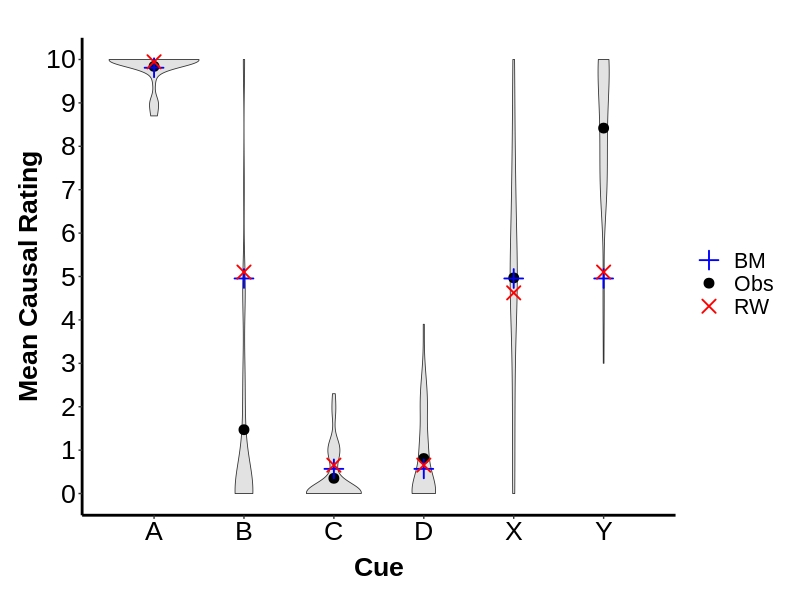
\includegraphics[width=\columnwidth]{fig1.jpg}
\caption{Predicted versus observed test stage ratings for unmodified Rescorla
\& Wagner (RW) model, and Bush \& Mosteller (BM) model, against observed
data (Obs), following A+/AX+ B-/BY+ C-/CD- training. The violin plot
represents the distribution of the observed data using a method
comparable to Hintze \& Nelson (1998). The distribution of the predicted
data is not represented, as it was negligible.}
\end{figure}

\subsection{Modifying the Rescorla-Wagner model}

The Rescorla and Wagner (1972) model was originally developed as an
account of non-human animal learning. In that context, it makes sense
for the associative strength of cues to start at zero, because animals
such as rats would not have learned a response to previously
non-encountered cues. However, in our human blocking experiment, it
seems unlikely that a novel cue would produce an associative strength of
zero, since participants would lack sufficient information to determine
whether or not it is a cause of stomach ache. An associative strength of
zero should result in the production of low causal ratings, so a more
intuitive response would be for participants to provide novel cues with
an intermediate rating (for example 5 on a scale running from 0-10),
reflecting their uncertainty about their causal status. This is
supported by Spicer et al. (under review), in an experiment where a
novel cue at test was assigned an intermediate rating of 4.85 on a 0-10
likelihood scale. Negative associative strengths are also possible,
meaning that a value between 0 and 1 is not strictly intermediate.
However, the acquisition of negative associative strengths to cues (i.e.
inhibition) is difficult to achieve in human predictive learning
experiments using foods as cues (e.g. Zaksaite \& Jones, 2019). This is
presumably because eating one food would not typically prevent an
allergic reaction from being caused by another food. Therefore, an
associative strength of 0.5 was regarded as an appropriate
representation of participants' uncertainty.

We conducted our model fitting procedure on the blocking data a second
time, using modified versions of both models, in which the initial
associative strength of cues was an additional parameter for
optimisation. The concept of non-zero starting associative strengths is
not in itself novel (e.g. Gluck \& Bower, 1988); for example, non-zero
initial strengths have been used to represent pre-training (Miller \&
Shettleworth, 2007, Dupuis \& Dawson, 2013). However, using them as a
representation of human uncertainty is novel. Moreover, the requirement
of intermediate (non-zero) strengths in order for the Rescorla and
Wagner (1972) model to explain a blocking experiment more effectively
than the Bush and Mosteller (1951) model would be a novel finding. This
concept has been discussed informally (e.g. Zaksaite, 2017) but not
formally simulated. We chose to fully explore the parameter space,
rather than setting this value at 0.5, since if a substantially
different value provided the best fit, it would indicate that our
proposal was incorrect.

\subsection{Results from modified model implementations}

If the Rescorla and Wagner (1972) model is modified so that the starting
associative strength can be something other than zero, then it accounts
for the results of our blocking experiment better than the equivalently
modified Bush and Mosteller (1951) model. The modified Bush-Mosteller
model produced a mean error of 0.04 and an $R^2$ of 0.93.
The modified Rescorla-Wagner model produced a mean error of 0.01 and an
$R^2$ of 1.00, therefore producing less error and a
better adequacy of fit. Whilst the modified Bush-Mosteller model
provided a better fit than the unmodified version (e.g. it predicted a
difference between B and Y, because B declines in associative strength
during the B- trials in Stage 1, while Y starts at an intermediate
strength in Stage 2), the lack of a summed error term does not allow it
to predict blocking. Figure 2 shows the predicted versus observed test
cue ratings for both models.

\begin{figure}[t!]
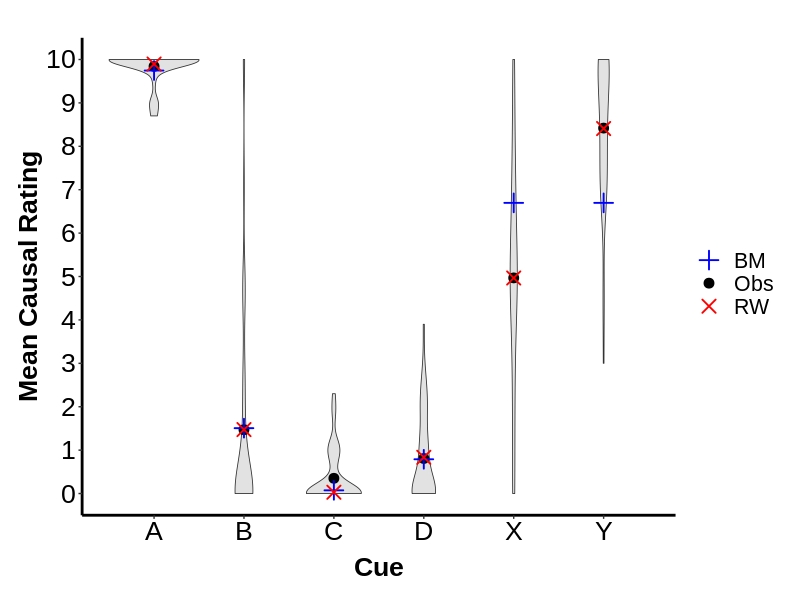
\includegraphics[width=\columnwidth]{fig2.jpg}
\caption{Predicted versus observed test
stage ratings for modified Rescorla \& Wagner (RW) model, and Bush \&
Mosteller (BM) model, against observed data (Obs), following A+/AX+
B-/BY+ C-/CD- training. The violin plot represents the distribution of
the observed data.}
\end{figure}

As predicted, the best fitting initial associative strengths were at an
intermediate value for both models (0.45 for Bush-Mosteller and 0.43 for
Rescola-Wagner). This finding is consistent with the idea that
participants assign intermediate ratings to cues that have an unknown
causal status.

\section{Simulation set 2: Redundancy effect}

Next, we investigated whether our modified Rescorla and Wagner (1972)
model could adequately capture a further psychological phenomenon that
the unmodified model cannot; the redundancy effect (e.g. Jones \&
Zaksaite, 2018; Jones et al., 2019; Uengoer et al., 2013; Uengoer et
al., 2019). The training stage of a redundancy effect design
incorporates blocking (A+ AX+) and a simple discrimination (BY+ CY-).
Cue Y is referred to as an uncorrelated cue, because it appears in both
a causal and a non-causal compound. The redundancy effect is the
observation of X being rated as a more likely cause of the outcome than
Y. The blocked cue (X) is typically given intermediate causal ratings at
test, while the uncorrelated cue (Y) is typically given low causal
ratings.

Rather than using a previously published data set, we collected a set of
redundancy effect data (see Supplementary Materials). This was to
provide a more diagnostic test stage than simply asking participants to
provide likelihood ratings for the five single cues (A, B, C, X, Y). We
also asked them to provide ratings for each of the ten possible compound
cue pairs (that can be produced using these five individual cues).
Importantly, the training participants received was equivalent to the
training used in previous redundancy effect demonstrations (A+ AX+ BY+
CY-). However, having a wider set of cues in the test Stage meant that
the two models could be `stretched', by being required to fit a more
complex set of test data.

\subsection{Results from modified model implementations}

The modified Rescorla and Wagner (1972) model produced a mean error of
0.02 and an $R^2$ of 0.96, indicating a good account of
the dataset. This was better than the unmodified model, which produced a
mean error of 0.03 and and $R^2$ of 0.83. The modified
Bush and Mosteller (1951) model provided a poor account of the dataset
($R^2$ of 0.63), with no discernible improvement on the
unmodified model ($R^2$ of 0.62); this suggests that our
modification is not simply leading to over-fitting from the inclusion of
an additional parameter. Figure 3 shows the predicted versus observed
test data for the modified models. The modified Rescorla-Wagner model
captured the redundancy effect, although the size of the effect was
somewhat underestimated. The Bush-Mosteller model accounted for the
redundancy effect itself, but not the full set of test data.


\begin{figure}[t!]
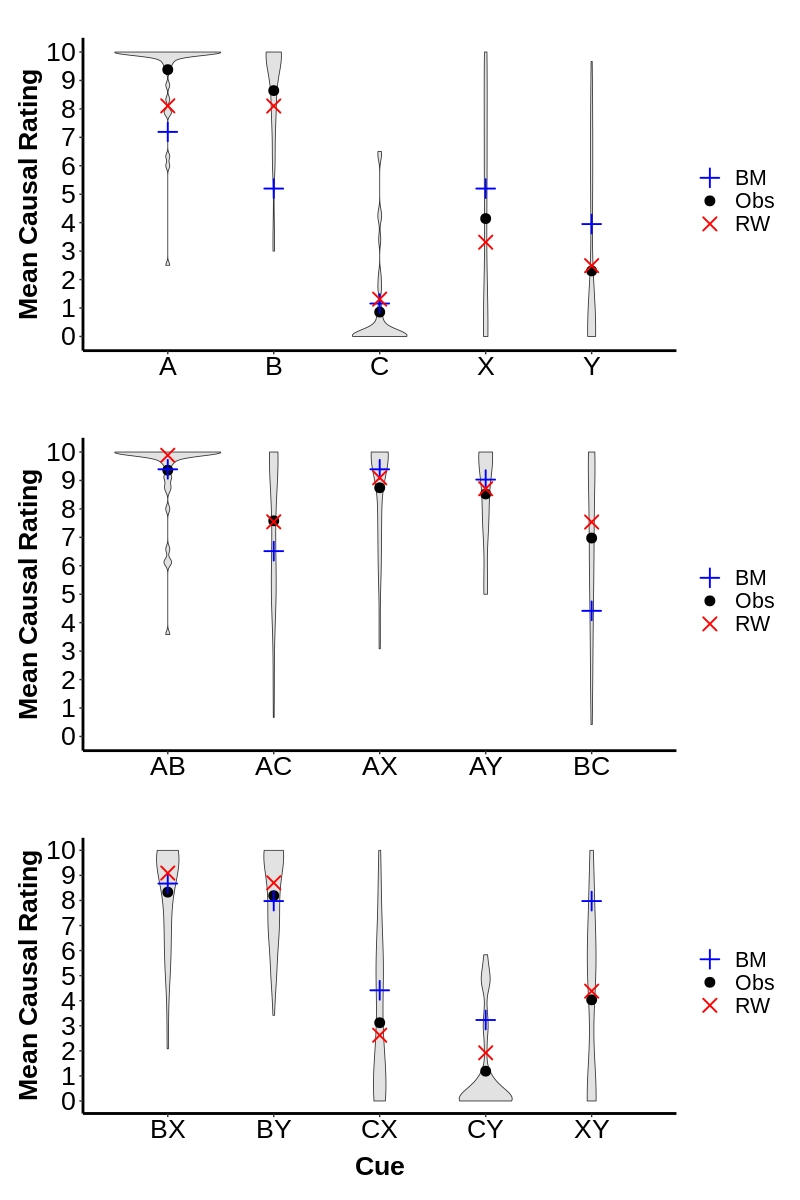
\includegraphics[width=\columnwidth]{fig3.jpg}
\caption{Predicted versus observed test stage ratings for modified Rescorla \&
Wagner (RW) model, and Bush \& Mosteller (BM) model, against observed
data (Obs), following A+ AX+ BY+ CY- training. The violin plot
represents the distribution of the observed data.}
\end{figure}

As with the blocking simulation, the best fitting initial associative
strength was an intermediate value (0.62). It is notable that the value
was slightly higher than for the blocking data. This could be because
the outcome base rate during training (i.e. the proportion of trial
types resulting in stomach ache versus no stomach ache) was higher.
There is evidence from Jones et al. (2019) that participants' causal
ratings of cues they are uncertain about are sensitive to the outcome
base rate. If starting associative strength is an adequate
representation of uncertainty about the status of novel cues, then the
best-fitting starting associative strength should change in line with
the outcome base rate. It is possible to test this idea by model fitting
on a dataset in which the outcome base rate has been experimentally
manipulated. This was the basis of our final model fitting procedure.

\section{Simulation set 3: Redundancy effect base rate manipulation}

A suitable dataset was already available for the final model fitting
procedure. Jones et al. (2019) reported a redundancy effect experiment,
in which the outcome base rate was varied between different groups of
human participants. Full experimental details are available in their
paper and a brief summary is included in our Supplementary Materials.
The test-stage likelihood ratings assigned to blocked cues were shown to
vary in line with the outcome base rate. In both groups, the redundancy
effect was observed, because the blocked cue (X) was assigned higher
ratings than the uncorrelated cue (Y). However, the rating for X was
higher in the high base rate group. The manipulation was achieved by
adding additional cues, so that either 25\% or 75\% of training trials
resulted in stomach ache. To test the prediction that starting
associative strength is sensitive to experimental base rate, this
parameter was allowed to vary by condition. None of the other parameters
were allowed to vary by condition. If correct, the modified Rescorla and
Wagner (1972) model should provide a good fit to all the test cues for
both groups, with a higher best-fitting initial associative strength in
the 75\% group than in the 25\% group.

\subsection{Results from modified model implementation}

The modified Rescorla and Wagner (1972) model produced a mean error of
0.03. The $R^2$ was 0.98 in both the 25\% and 75\% base
rate groups, indicating a good fit. As predicted, the best fitting
initial associative strength was higher in the high base rate group
(0.51) than in the low base rate group (0.39). Our initial associative
strength parameter appears to provide one reasonable way of representing
participants' uncertainty about the causal status of novel cues. Of
course, real participants, unlike our simulation, need to experience at
least a few trials in order to become sensitive to base rate. Thus,
using initial starting weights to model the effects of outcome base rate
is necessarily a simplification of the mental operations involved.
Figure 4 shows the predicted versus observed test stage ratings for the
25\% and 75\% groups. The modified Rescorla-Wagner model was able to
capture the redundancy effect in both conditions. It also captured the
labile nature of blocked cue X, although the effect of the base rate on
X is slightly underestimated.

\begin{figure}[t!]
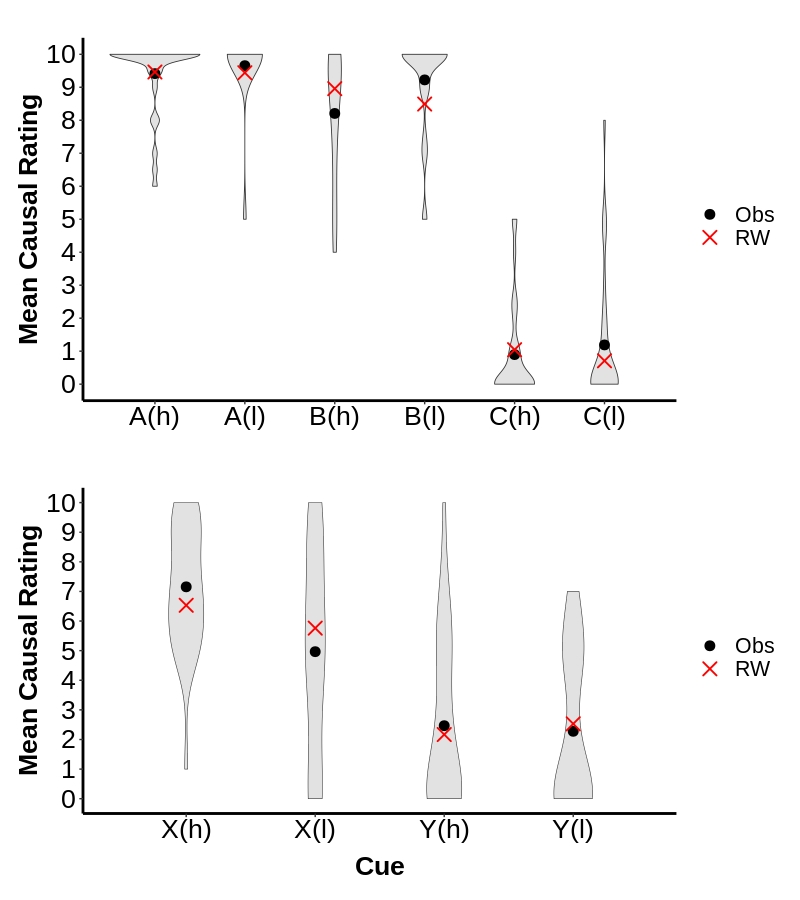
\includegraphics[width=\columnwidth]{fig4.jpg}
\caption{Predicted versus observed test stage ratings for modified
Rescorla-Wagner (RW) model, against observed data (Obs), fitting to the
high (h) and low (l) base rate groups, following A+ AX+ BY+ CY- training
(intermixed with additional cues used to manipulate the base rate). The
violin plot represents the distribution of the observed data.}
\end{figure}

\section{General Discussion}

\subsection{Summary of findings}

Contrary to intuition, the unmodified
Rescorla and Wagner (1972) model provides no better an account of a
standard forward cue-competition blocking experiment than the Bush and
Mosteller (1951) model. However, if the former is modified, such that
the initial associative strength of cues can be an intermediate value,
then it does provide a better account than the equivalently modified
Bush-Mosteller model. While the Rescorla-Wagner model can explain basic
cue competition, it needs modification to be able fit the full
experimental results; and can then do so almost perfectly. The modified
Rescorla-Wagner model is also able to adequately account for the
redundancy effect (e.g. Uengoer et al, 2013), which the unmodified model
cannot. Additionally, the initial associative strength of the simulated
cues was shown to vary with the outcome base rate, supporting the
suggestion that intermediate initial associative strengths can be used
to represent uncertainty about novel cues. This is consistent with the
experimental findings of Jones et al. (2019), in that the likelihood
ratings assigned to cues with an uncertain causal status are influenced
by the outcome base rate. The best fitting initial associative strength
may also be influenced by the range of plausible associative strengths
within specific experimental scenarios. The experiments in this paper
all used a food allergy scenario, in which inhibition was unlikely,
bounding plausible associative strengths between 0 and 1. However, in a
scenario where inhibition is possible, associative strengths could range
from -1 to +1, making 0 the intermediate value. This could be tested
with a modified scenario (e.g. pharmaceutical drugs as cues), and a
design with some cues explicitly trained as inhibitors.

\subsection{Fitting the full results}

We have taken the position in this
article that it is important to fit the full results of an experiment,
rather than a hand-selected subset of cues. One might argue that this
approach could lead to trivial features of the experiment becoming
crucial in model comparison. However, it seems to us that a cue cannot
be both theoretically trivial \emph{and} crucial in model comparison.
For example, a cue might be theoretically trivial in the sense that all
models inevitably predict responding to that cue correctly. If that is
the case, then this cue cannot affect which of two competing models best
fits the data -- inclusion of the trivial cue cannot change the winner
of the contest. Conversely, a cue might affect the outcome of a model
comparison to the extent that different models make different
predictions about it. Such a cue is of theoretical importance, as it
allows us to distinguish between different models. One might argue that
experiments sometimes include cues that the models were not intended to
explain, and thus including those cues in a model comparison is unfair.
In such cases, it seems to us that the onus is on the proponents of the
models to specify which sub-components of an experiment the model should
not be expected to explain.

\subsection{Other accounts}

Vogel and Wagner (2016) suggested an
alternative approach using the Rescorla and Wagner (1972) model that
also accommodates the redundancy effect. In their approach, common
elements are added to the stimulus representation. While this approach
has been shown to accommodate the basic redundancy effect, there is
evidence that it cannot adequately account for the effect of varying the
outcome base rate on the redundancy effect (Jones et al., 2019).
Nevertheless, further investigation of both approaches, across a range
of phenomena, would be a fruitful direction for future research. The
importance of making broad relative adequacy comparisons of models has
been previously emphasised within the literature (Wills \& Pothos, 2012;
Wills et al., 2017). Further research could also investigate a role for
context in explaining the data (e.g. Bouton, 2010). Both minor
experimental variations (e.g. different types of control used for
blocking), and more substantially different designs, might produce
different model comparison results. It would also be useful to know
whether other associative models could account for these results (e.g.
Gershman, 2015; Kokkola et al., 2019; McLaren \& Mackintosh (2000,
2002); Schmajuk et al., 1996; Wagner, 1981); with or without
modifications to the initial associative strengths.

\subsection{Extended test sets}

Instead of model fitting to a redundancy
effect dataset only incorporating five single cues at test, we used an
expanded set of test cues (Simulation Set 2). Given the high adequacy of
fit ($R^2$ value 0.96) observed for the modified Rescorla
and Wagner (1972) model, a further fitting procedure conducted on a
dataset incorporating only five single test cues could not produce a fit
any worse than this. Whilst there is some scope for the Bush and
Mosteller (1951) model to produce a better fit with fewer test cues, the
best this could result in is both models producing a comparably good fit
as each other. In this scenario, the modified Rescorla-Wagner model
would still provide the best account across the phenomena considered in
this paper. We suggest that future predictive learning experiments
should incorporate extended test sets, since this may provide a more
diagnostic test of the relative adequacy of models. We welcome further
debate and discussion of this suggestion.

\subsection{Open science for formal models}

Our simulations also
demonstrate the value of thoroughly investigating the parameter space of
formal models. Formal simulations are becoming more common in the study
of human predictive learning, but one possible barrier is the apparent
lack of a common open framework, in which models, phenomena and
simulations can be easily assessed and compared. However, options are
available, such as ALTSim (Thorwart et al. 2009). ALTSim does not allow
for parameter space optimisation, but it does allow initial associative
strengths to be set to values other than zero. The model implementations
reported in the current paper used the free and open source package
\emph{catlearn }(Wills et al., 2019), which is available to download in
the open-source R environment (R Core Team, 2018). \emph{catlearn}
includes a number of model implementations, including Rescorla and
Wagner (1972), Bush and Mosteller (1951), EXIT (Kruschke, 2001), and
COVIS (Ashby et al., 1998). It is an extensible framework to which more
models can be added.

\subsection{Conclusion}

Our simulations show that intermediate starting
associative strengths are needed for the Rescorla and Wagner (1972)
model to fit the results of a simple forward cue competition experiment
better than the Bush and Mosteller (1951) model. Contrary to intuition,
both models perform equally poorly in the absence of this change.
Furthermore, this simple change allows the Rescorla-Wagner model to
account for both the redundancy effect, and the effect of base rate on
the redundancy effect.

\section*{Author contributions}

\textbf{SGS} (lead author): Co-contributor to the rationale, design of the
experiments, and theoretical basis of the simulations. Programmed the
simulations and experiments. Co-programmed the model implementations. Collected
and analysed the data as part of his Ph.D.  Wrote up the simulations and
experiments. \textbf{AJW}: Co-contributor to the rationale, design of the
experiments, and theoretical basis of the simulations. Consulted on analysis
and write up of simulations and experiments as Ph.D.  supervisor.
\textbf{PMJ}: Contributed to rationale, interpretation and write up as
Ph.D. supervisor.
\textbf{CJM}: Contributed to interpretation and write up as
co-author.
\textbf{LD}: Co-programmed the model implementations.

\section*{References}

\begin{hangparas}{1em}{1}

Ashby, F. G., Alfonso-Reese, L. A., \& Waldron, E. M. (1998). A
neuropsychological theory of multiple systems in category learning.
\emph{Psychological Review, 105}(3), 442-481.
\url{https://doi.org/10.1037/0033-295x.105.3.442}

Bouton, M. E. (2010).~\emph{\emph{The multiple forms of "context" in
associative learning theory.}}~In B. Mesquita, L. F. Barrett, \& E. R.
Smith (Eds.),~\emph{\emph{The mind in context}}~(p. 233--258). Guilford
Press. \url{http://doi.org/10.1101/lm.493707}

Bush, R. R., \& Mosteller, F. (1951). A mathematical model for simple
learning. \emph{Psychological Review, 58}, 313--323.
\url{https://doi.org/10.1007/978-0-387-44956-2_12}

Dickinson, A., Shanks, D., \& Evenden, J. (1984). Judgement of
act-outcome contingency: The role of selective attribution. \emph{The
Quarterly Journal of Experimental Psychology}, \emph{36}(1), 29-50.
\url{https://doi.org/10.1080/14640748408401502}

Dupuis, B., \& Dawson, M. R. (2013). Differentiating models of
associative learning: Reorientation, superconditioning, and the role of
inhibition.~\emph{Journal of Experimental Psychology: Animal Behavior
Processes},~\emph{39}(3), 273. \url{https://doi.org/10.1037/a0032174}

Gershman, S. J. (2015). A unifying probabilistic view of associative
learning. \emph{PLoS Comput Biol}, \emph{11}(11).
\protect\hypertarget{anchor-1}{}{}\url{https://doi.org/10.1371/journal.pcbi.1004567}

Gluck, M. A., \& Bower, G. H. (1988). From conditioning to category
learning: an adaptive network model. \emph{Journal of Experimental
Psychology: General, 117}(3), 227-247.
\url{https://doi.org/10.1037/0096-3445.117.3.227}

Jones, P. M., \& Zaksaite, T. (2018). The redundancy effect in human
causal learning: no evidence for changes in selective attention.
\emph{Quarterly Journal of Experimental Psychology, 71}(8), 1748-1760.
\url{https://doi.org/10.1080/17470218.2017.1350868}

Jones, P. M., Zaksaite, T., \& Mitchell, C. J. (2019). Uncertainty and
blocking in human causal learning. \emph{Journal of Experimental
Psychology: Animal Learning and Cognition, 45}(1), 111-124.
\url{https://doi.org/10.1037/xan0000185}

Kamin, L. J. (1969). Selective association and conditioning. In N. J.
Mackintosh \& W. K. Honig (Eds.), \emph{Fundamental Issues in
Associative Learning} (pp. 42--64). Halifax, Canada: Dalhousie
University Press.

Kokkola, N. H., Mondragón, E., \& Alonso, E. (2019). A double error
dynamic asymptote model of associative learning. \emph{Psychological
review}, \emph{126}(4), 506. \url{https://doi.org/10.1101/210674d}

Kruschke, J. K. (2001). Toward a unified model of attention in
associative learning. \emph{Journal of mathematical psychology},
\emph{45}(6), 812-863. \url{https://doi.org/10.1006/jmps.2000.1354}

McLaren, I. P. L., \& Mackintosh, N. J. (2000). An elemental model of
associative learning: I. Latent inhibition and perceptual learning.
\emph{Animal Learning \& Behavior}, \emph{28}(3), 211-246.
\url{https://doi.org/10.3758/BF03200258}

McLaren, I. P. L., \& Mackintosh, N. J. (2002). Associative learning and
elemental representation: II. Generalization and discrimination.
\emph{Animal learning \& behavior}, \emph{30}(3), 177-200.
\url{https://doi.org/10.3758/BF03192828}

Miller, R. R., \& Matute, H. (1996). Biological significance in forward
and backward blocking: Resolution of a discrepancy between animal
conditioning and human causal judgment. \emph{Journal of Experimental
Psychology: General}, \emph{125}(4), 370-386.
\url{https://doi.org/10.1037/0096-3445.125.4.370}

Miller, N. Y., \& Shettleworth, S. J. (2007). Learning about
environmental geometry: An associative model. \emph{\emph{Journal of
Experimental Psychology: Animal Behavior Processes, 33}}(3), 191--212.
\href{https://doi.org/10.1037/0097-7403.33.3.191}{https://doi.org/}\href{https://doi.org/10.1037/0097-7403.33.3.191}{10.1037/0097-7403.33.3.191}

Mitchell, C. J., \& Lovibond, P. F. (2002). Backward and forward
blocking in human electrodermal conditioning: Blocking requires an
assumption of outcome additivity. \emph{The Quarterly Journal of
Experimental Psychology Section B}, 55(4b), 311-329.
\url{https://doi.org/10.1080/02724990244000025}


Nosofsky, R. M., Gluck, M. A., Palmeri, T. J., McKinley, S. C., \&
Glauthier, P. (1994). Comparing modes of rule-based classification
learning: A replication and extension of Shepard, Hovland, and Jenkins
(1961). \emph{Memory \& cognition}, \emph{22}, 352-369.

Peirce, J. W. (2007). PsychoPy - Psychophysics software in Python.
\emph{\emph{Journal of Neuroscience Methods,}
}\textbf{\emph{\textbf{162}}\textbf{(1:2)}}, 8-13.
\href{http://www.psychopy.org/}{\emph{www.psychopy.org}}. (Version
1.90.3). \url{https://doi.org/10.1016/j.jneumeth.2006.11.017}

R Core Team. (2018). \emph{R: A language and environment for statistical
computing}. \href{http://www.r-project.org/}{\emph{www.r-project.org}}.
(Version 3.5.3)

Rescorla, R. A., and Wagner, A. R. (1972). A theory of Pavlovian
conditioning: Variations in the effectiveness of reinforcement and
nonreinforcement. In A. H. Black \& W. F. Prokasy (Eds.),
\emph{Classical conditioning II: Current theory and research }(pp.
64-99). New York, NY: Appleton-Century-Crofts.
\url{https://doi.org/10.1016/0023-9690(71)90002-6}

Schmajuk, N. A., Lam, Y.-W., \& Gray, J. A. (1996). Latent inhibition: A
neural network approach. \emph{\emph{Journal of Experimental Psychology:
Animal Behavior Processes, 22}}(3), 321--349.
\href{https://psycnet.apa.org/doi/10.1037/0097-7403.22.3.321}{https://doi.org/10.1037/0097-7403.22.3.321}

Shanks, D. R. (1985). Forward and backward blocking in human contingency
judgement. \emph{The Quarterly Journal of Experimental Psychology
Section B}, 37(1b), 1-21.
\url{https://doi.org/10.1080/14640748508402082}

Spicer, S. G., Mitchell, C. J., Wills, A. J., Blake. K. L., and Jones,
P. M. (under review). Theory protection: do humans protect existing
associative links?. \emph{Journal of Experimental Psychology: Animal
Learning and Cognition}.

Thorwart, A., Schultheis, H., König, S. \& Lachnit, H. (2009). ALTSim: A
MATLAB simulator for current associative learning theories.
\emph{Behavior Research Methods, 41}, 29-34.
\url{https://doi.org/10.3758/brm.41.1.29}

Uengoer, M., Lotz, A., Pearce, J. M., (2013). The fate of redundant cues
in human predictive learning. \emph{Journal of Experimental Psychology:
Animal Behaviour Processes, 39}(4), 323-333.
\url{https://doi.org/10.1037/a0034073}

Uengoer, M., Dwyer, D. M., Koenig, S., \& Pearce, J. M. (2019). A test
for a difference in the associability of blocked and uninformative cues
in human predictive learning. \emph{Quarterly Journal of Experimental
Psychology}, \emph{72}(2), 222--237.

Wagner, A. R. (1981). SOP: A model of automatic memory processing in
animal behavior. \emph{Information processing in animals: Memory
mechanisms}, \emph{85}, 5-47.
\href{https://doi.org/10.1037/024459}{https://doi.org/10.1037/024459 }

Wills, A. J., \& Pothos, E. M. (2012). On the adequacy of current
empirical evaluations of formal models of categorization.
\emph{Psychological bulletin}, \emph{138}(1), 102-125.
\url{https://doi.org/10.1037/a0025715}

Wills, A. J., O'Connell, G., Edmunds, C. E., \& Inkster, A. B. (2017).
Progress in Modeling Through Distributed Collaboration: Concepts, Tools
and Category-Learning Examples. \emph{In Psychology of Learning and
Motivation} (Vol. 66, pp. 79-115). Academic Press.
\url{https://doi.org/10.1016/bs.plm.2016.11.007}

Wills, A. J., Dome, L., Edmunds C. E., Honke, G., Inkster, A. B.,
Schlegelmilch, R., \& Spicer, S. G. (2019). catlearn: Formal
Psychological Models of Categorization and Learning.
\url{https://CRAN.R-project.org/package=catlearn}. \emph{R package
version 0.6.2.}

Zaksaite, G. (2017). The Redundancy Effect in Human Causal Learning:
Attention, Uncertainty, And Inhibition\emph{ (Doctoral dissertation,
University of Plymouth).}

Zaksaite, T., \& Jones, P. M. (2019). The redundancy effect is related
to a lack of conditioned inhibition: Evidence from a task in which
excitation and inhibition are symmetrical. \emph{Quarterly Journal of
Experimental Psychology, 73}(2)\emph{, }260--278.
\url{https://doi.org/10.1177/1747021819878430}

\end{hangparas}

\end{document}

%%% Local Variables:
%%% mode: latex
%%% TeX-master: t
%%% End:
